%!TEX root = ../main.tex

\chapter{Project Guidelines}
\label{ch:project_guidelines}

\section{Deployment Plan}\label{sec:deployment-plan}
\subsection{Gantt Chart}\label{subsec:gantt-chart}
\begin{figure}[H]
    \centering
    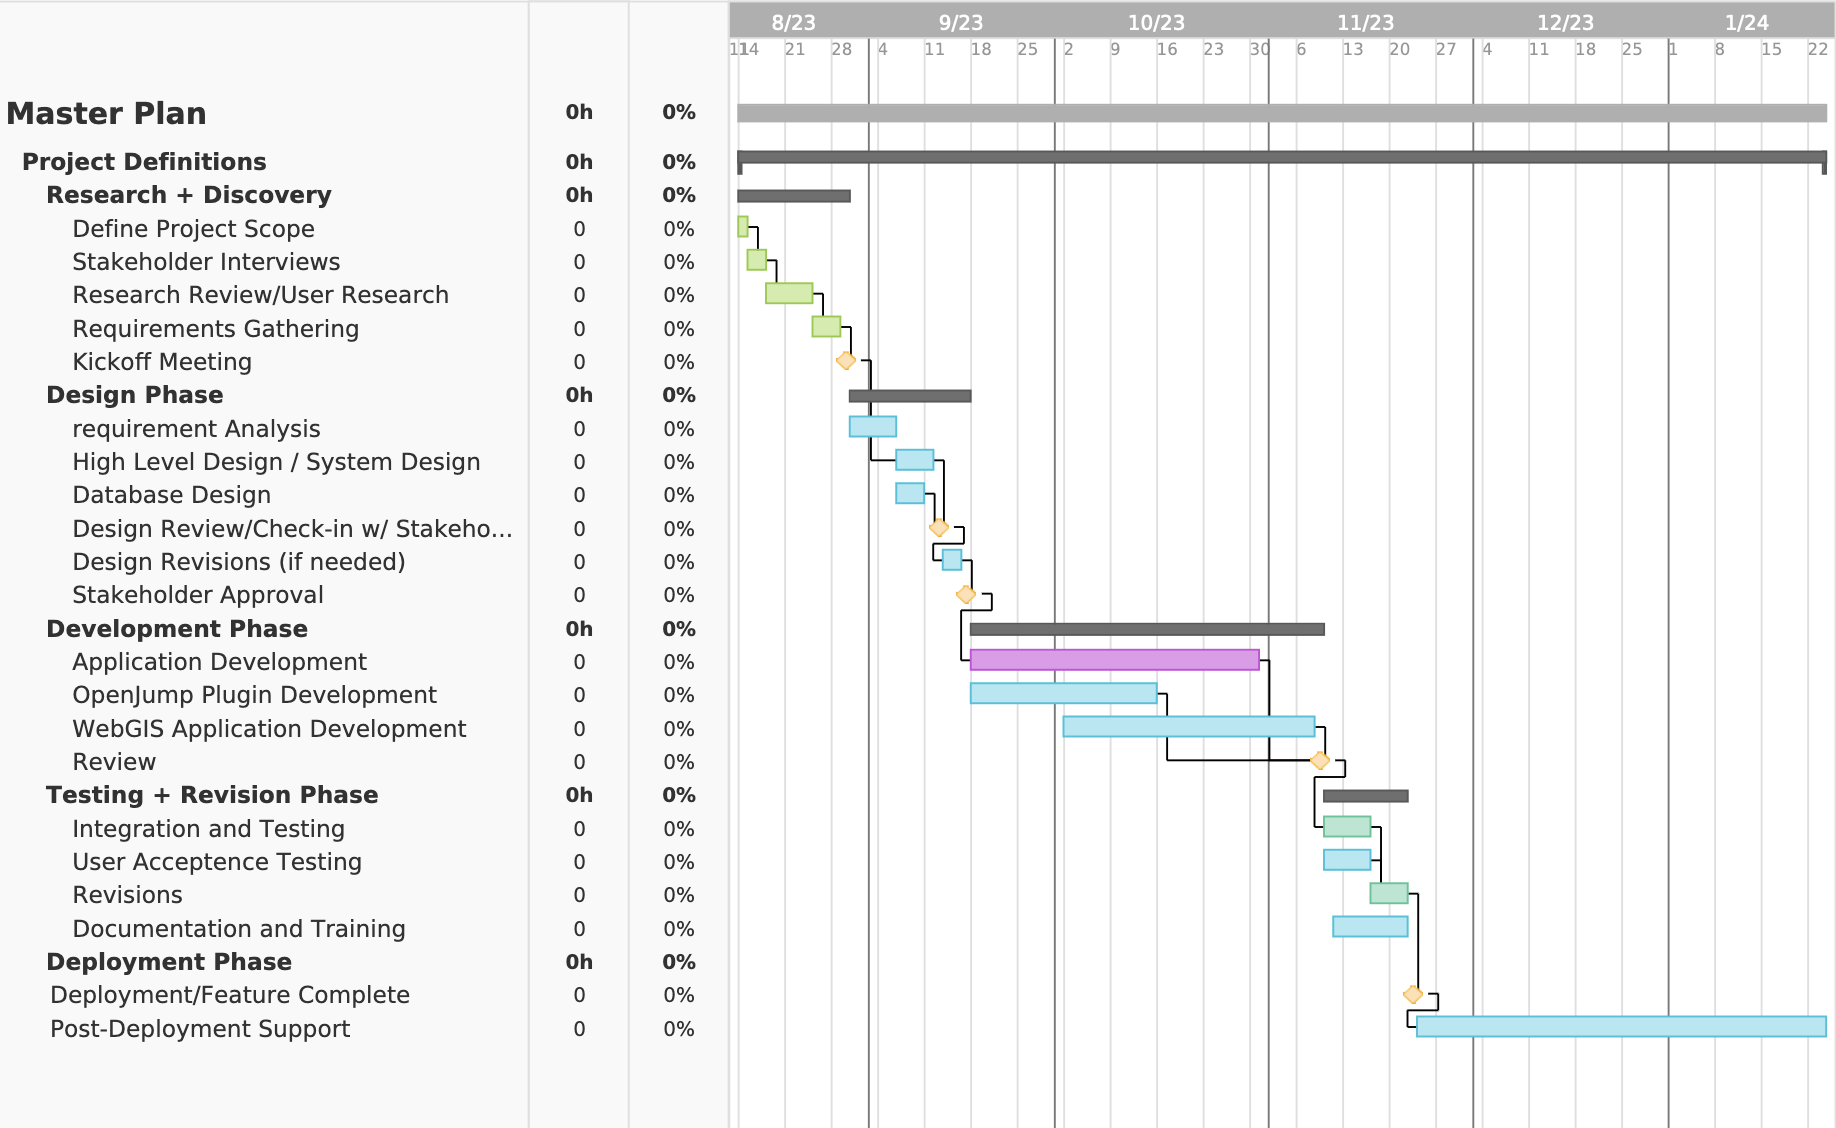
\includegraphics[width=\textwidth]{res/gantt_chart}
    \caption{Gantt Chart}
    \label{fig:gantt-chart}
\end{figure}

\subsection{Description of Gantt Chart}\label{subsec:description-of-gantt-chart}
The provided Gantt chart outlines the comprehensive timeline and sequence of tasks for the development of the GIS Master Plan Application. It serves as a visual representation of the project's progression, illustrating the major phases, activities, and their interdependencies. The Gantt chart begins with definig project scope, which entails initial planning and team coordination. It then segues into Requirements Analysis, System Design, and Database Design, where the project's fundamental groundwork is laid. Application Development, including the OpenJUMP Plugin and WebGIS Application, constitutes a significant portion of the timeline, culminating in Integration and Testing to ensure seamless operability. Subsequently, User Acceptance Testing, Documentation, and Training phases pave the way for a successful Deployment. Post-Deployment Support extends after deployment to address any issues and facilitate user adaptation. Finally, the project concludes with the Project Conclusion phase. This Gantt chart serves as a roadmap, enabling effective project management and tracking as the GIS Master Plan Application takes shape.

\subsection{Delivery Time}\label{subsec:delivery-time}
!! TODO
%The completion of the GIS Master Plan Application, as outlined in the Gantt chart, is projected to span approximately six months. The project is set to commence on September 1, 2023, with a target completion date of March 3, 2024. This timeframe accounts for the intricate stages of the project, including requirements analysis, system design, application development, testing, documentation, and deployment. It encompasses development, testing, training, and post-deployment support phases to ensure a robust and user-ready application. By adhering to this delivery time, the project aims to ensure the seamless and timely availability of the GIS Master Plan Application, meeting the needs of planners, technicians, and citizens in the Italian province of Fano.

\subsection{Benefits Evaluation}\label{subsec:benefits-evaluation}
This evaluation can be quantified through various metrics, including time saved in plan variant creation and approval, reduction in errors and inconsistencies, enhanced public participation, and increased efficiency in plan management. 
By streamlining workflows, providing real-time data access, and facilitating informed decision-making, the application will ultimately lead to more effective urban planning, reducing time-to-implementation and enabling better resource allocation.

\subsection{Benefits Identification}\label{subsec:benefits-identification}
Identifying benefits entails recognizing the tangible and intangible advantages that the GIS Master Plan Application will offer. For municipal planners, the application's streamlined plan variant management will expedite decision-making, enhance collaboration, and enable informed urban development strategies. Citizens will gain access to user-friendly tools that empower them to visualize and understand the Master Plan's implications, fostering transparent engagement and promoting better-informed decisions.
The application's capabilities to manage and analyze spatial data efficiently will lead to improved accuracy, reducing errors in plan management and minimizing resource wastage.

\section{Economic Quantification of the Benefits}\label{sec:economic-quantification-of-the-benefits}
In the realm of project management for the GIS Master Plan Application, economic quantification of the benefits holds significant importance.
\linebreak

\textbf{Cost Savings and Efficiency}

One key economic benefit lies in cost savings and enhanced operational efficiency.
The streamlined plan variant management facilitated by the application will lead to reduced manual effort, shortened approval cycles, and minimized errors.
These efficiency gains translate into quantifiable cost reductions, including savings in personnel time, administrative overhead, and resource utilization.
Moreover, improved accuracy in plan management will reduce the costs associated with rectifying errors and addressing inconsistencies that might arise from traditional manual processes.
\linebreak

\textbf{Enhanced Civic Engagement and Decision-Making}

The application's capabilities to promote transparent public engagement and provide citizens with user-friendly tools for understanding the Master Plan's implications have significant economic implications as well.
Informed citizen participation can lead to more effective land use decisions, reducing the potential for legal disputes and costly reversals in development projects.
Additionally, by fostering greater community understanding and collaboration, the application can potentially attract investments and development opportunities, thus contributing positively to the local economy.
\linebreak

\textbf{Time-to-Implementation Reduction}

Another economic advantage lies in the reduction of time-to-implementation for plan variants.
The streamlined process enabled by the application can lead to faster plan approval, subsequently accelerating the execution of development projects.
This reduced time frame results in faster revenue generation for commercial and residential projects, positively impacting the economic growth of the municipality.
\linebreak

\textbf{Data-Driven Decision-Making}

The application's ability to provide real-time access to accurate spatial data supports data-driven decision-making.
This leads to better resource allocation, optimized land use strategies, and improved urban planning initiatives.
By maximizing the efficiency of projects and minimizing resource wastage, the application contributes to economic sustainability and growth.


\section{Cost Evaluation}\label{sec:cost-evaluation}
This process involves a comprehensive analysis of both project costs and ongoing operational expenses, ensuring transparency and informed decision-making regarding resource allocation.
\subsection{Project Costs}\label{subsec:project-costs}
These costs include personnel salaries, software and hardware acquisition, third-party services, licensing fees, development tools, and any associated training expenses.
Additionally, costs related to quality assurance and testing, documentation, user interface design, and project management tools are considered.
Accurate project cost evaluation provides a clear understanding of the investment required to bring the application to fruition, enabling effective budget planning and resource allocation.

TODO !! TABLE


\subsection{Running Costs}\label{subsec:running-costs}
The running costs encompass the ongoing operational expenses to maintain and sustain the GIS Master Plan Application.
These costs include hosting and server maintenance, cloud services, technical support, software updates, security measures, and system monitoring. 
User training, system administration, and regular data updates also contribute to running costs. 
By anticipating these ongoing expenses, project stakeholders can ensure the application's continuous functionality, user satisfaction, and alignment with the allocated budget.

TODO !! TABLE
